The past decade has witnessed a vast growth of intelligent robotic solutions for logistics and warehouse automation tasks, with the {\it Amazon Kiva} mobile robotic fulfillment system serving as a prime example~\cite{Enright:2011:OCA:2908675.2908681}.  Nevertheless, the completion of many tasks still rely on the use of repetitive human labor, such as for picking and packing of products and building customer orders.  In particular, tightly packing products that are picked from an unstructured pile, the focal task of this work, still remains primarily manual, even though it is integral to warehouse automation and manufacturing.

Packing objects to fit in confined spaces, such as a small shipping box as the one in Fig.~\ref{fig:new_setup} (left), is highly challenging. It can be argued that is more difficult than clearing clutter since packing requires placing objects in close vicinity to each other, in an ordered manner and also to be well aligned with the boundary of the container. This demands high levels of accuracy from the perception component as well as the manipulation strategy. Indeed, surprisingly little prior work seems to exist that explicitly addresses this problem, let alone using a simple, suction-based end-effector.

\rahul{
The current work was undertaken to address a pressing need outlined by industry partners at JD-X Research and Development Center. The criticality of robust, autonomous packing is reflected in the economic, and environmental savings from a reduction in packaging material, storage space, and shipping costs. Industry stakeholders motivated the problem in the context of order fulfilment and warehouse automation. The current work raises and addresses the research questions that can jump-start future industrial deployments. 
}


\begin{figure*}[t]
\centering
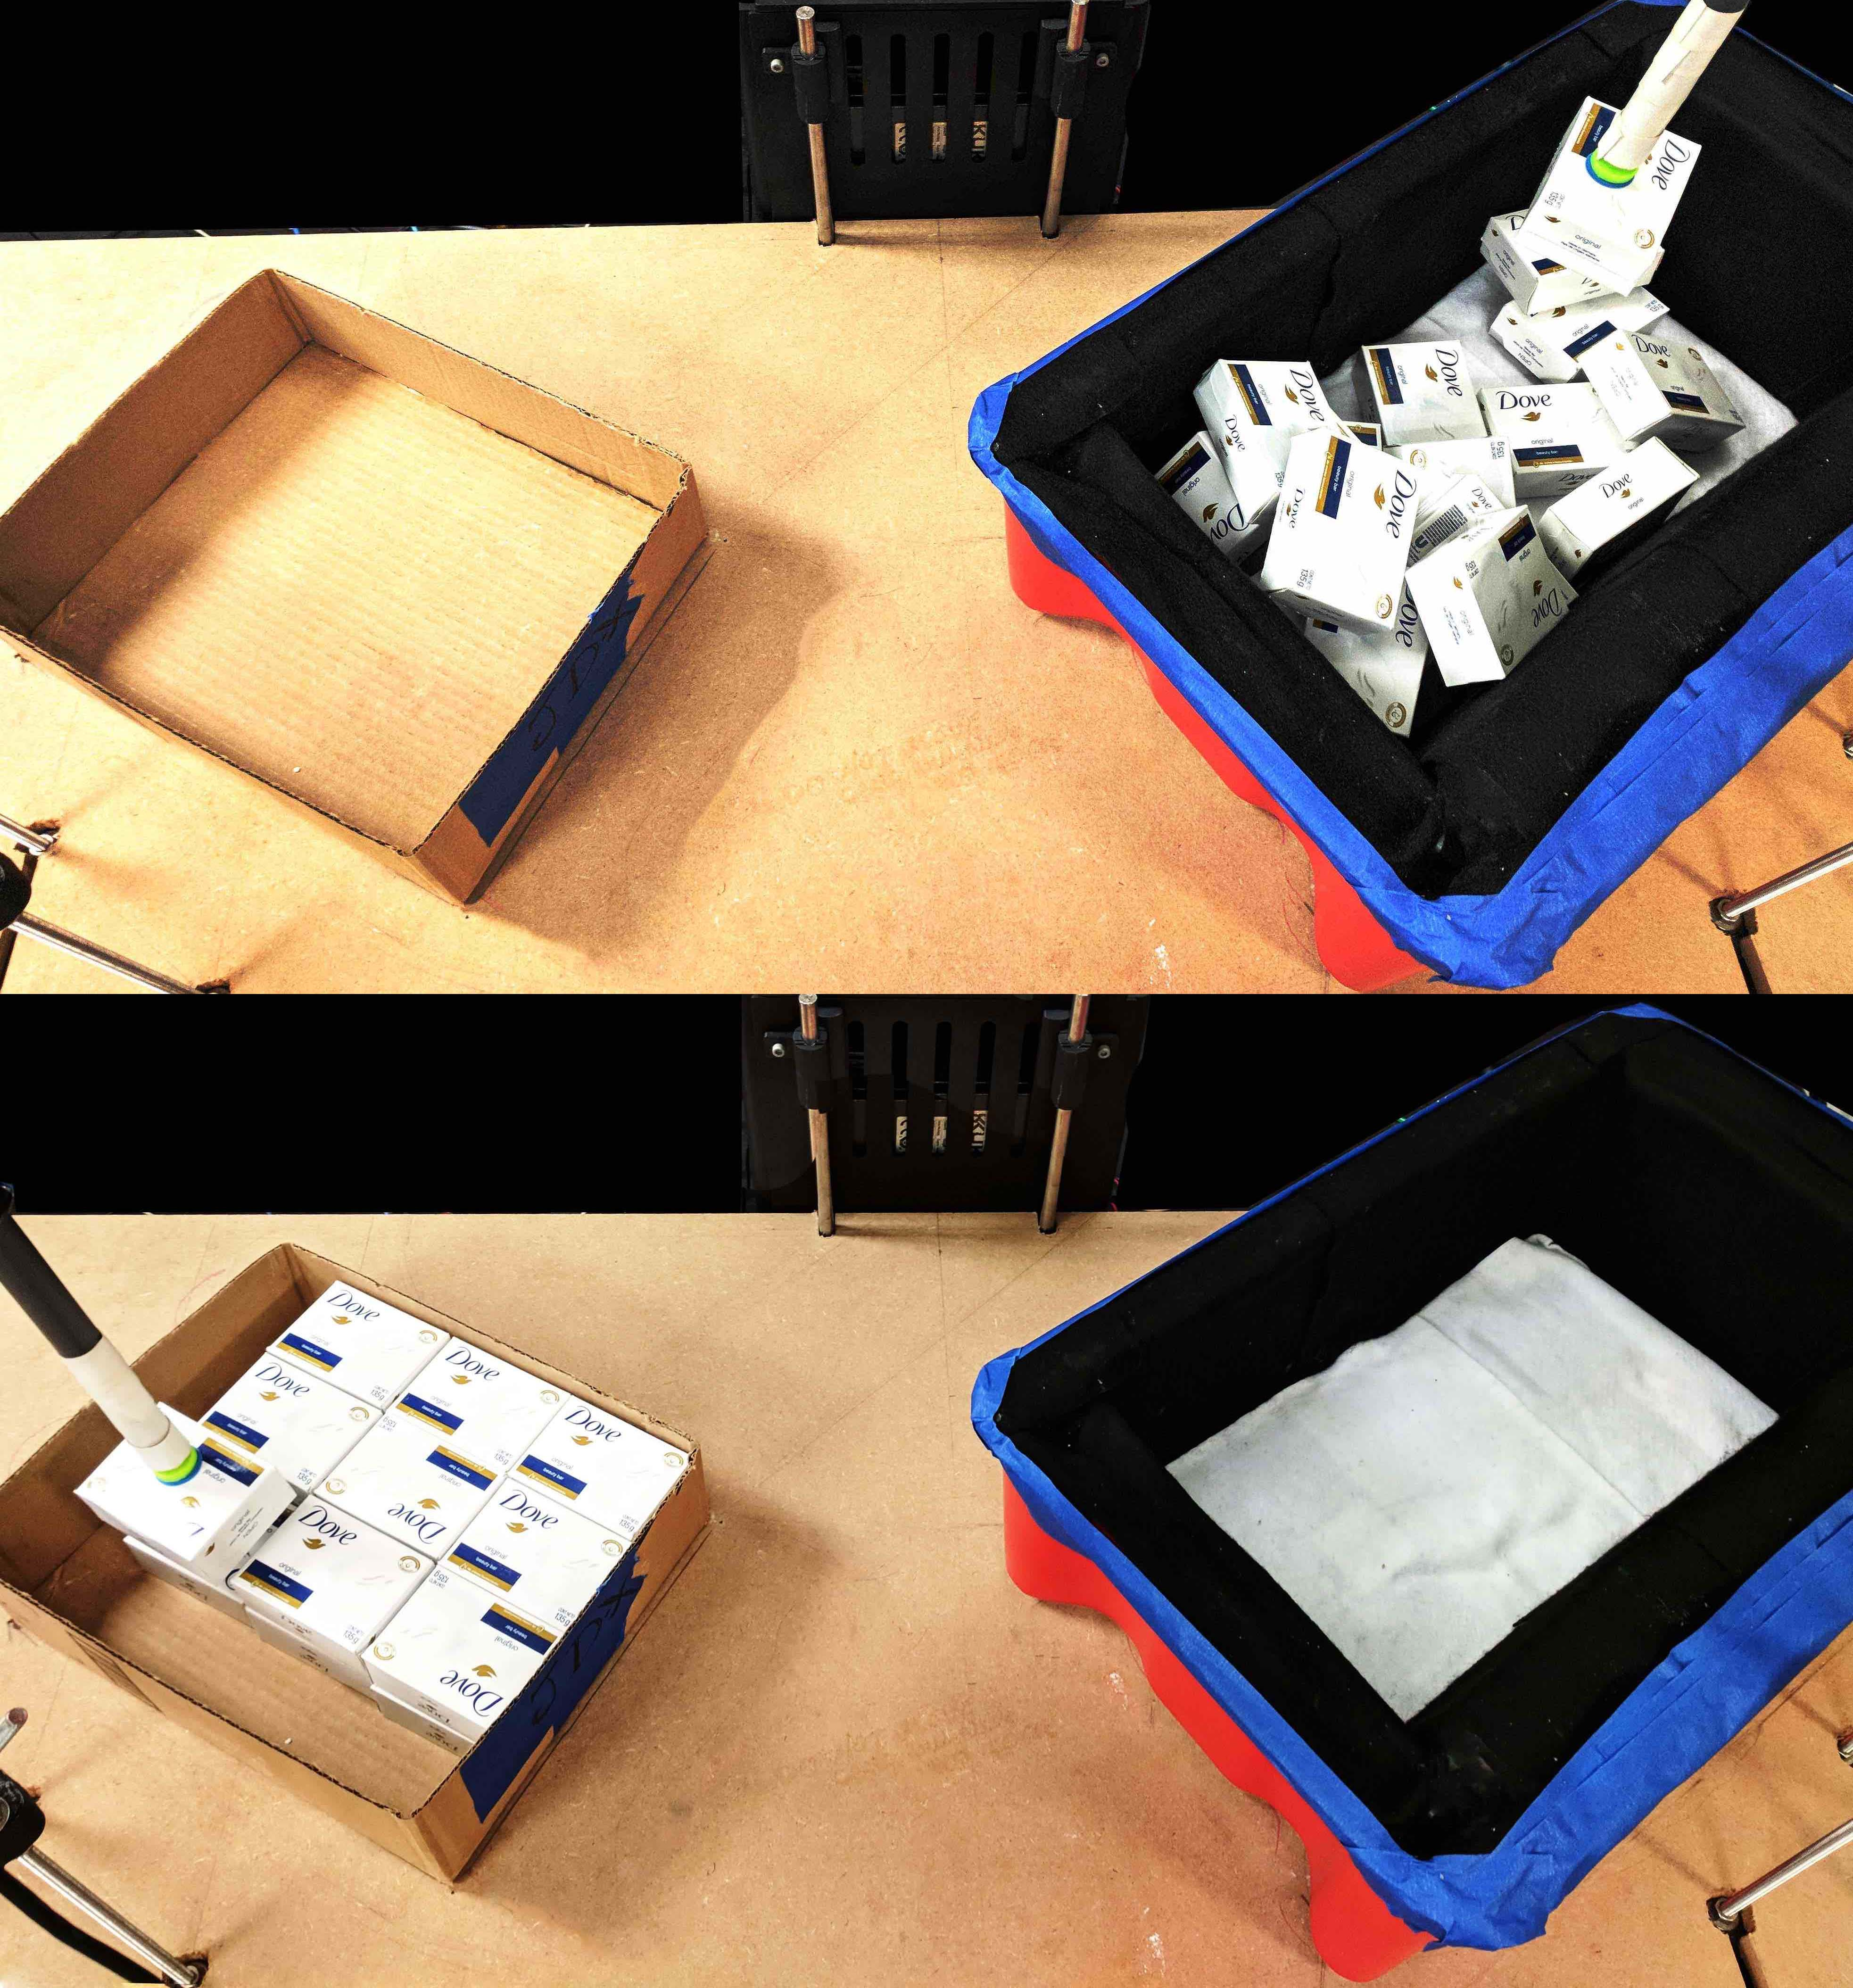
\includegraphics[height=2in]{Figures/initial_final}
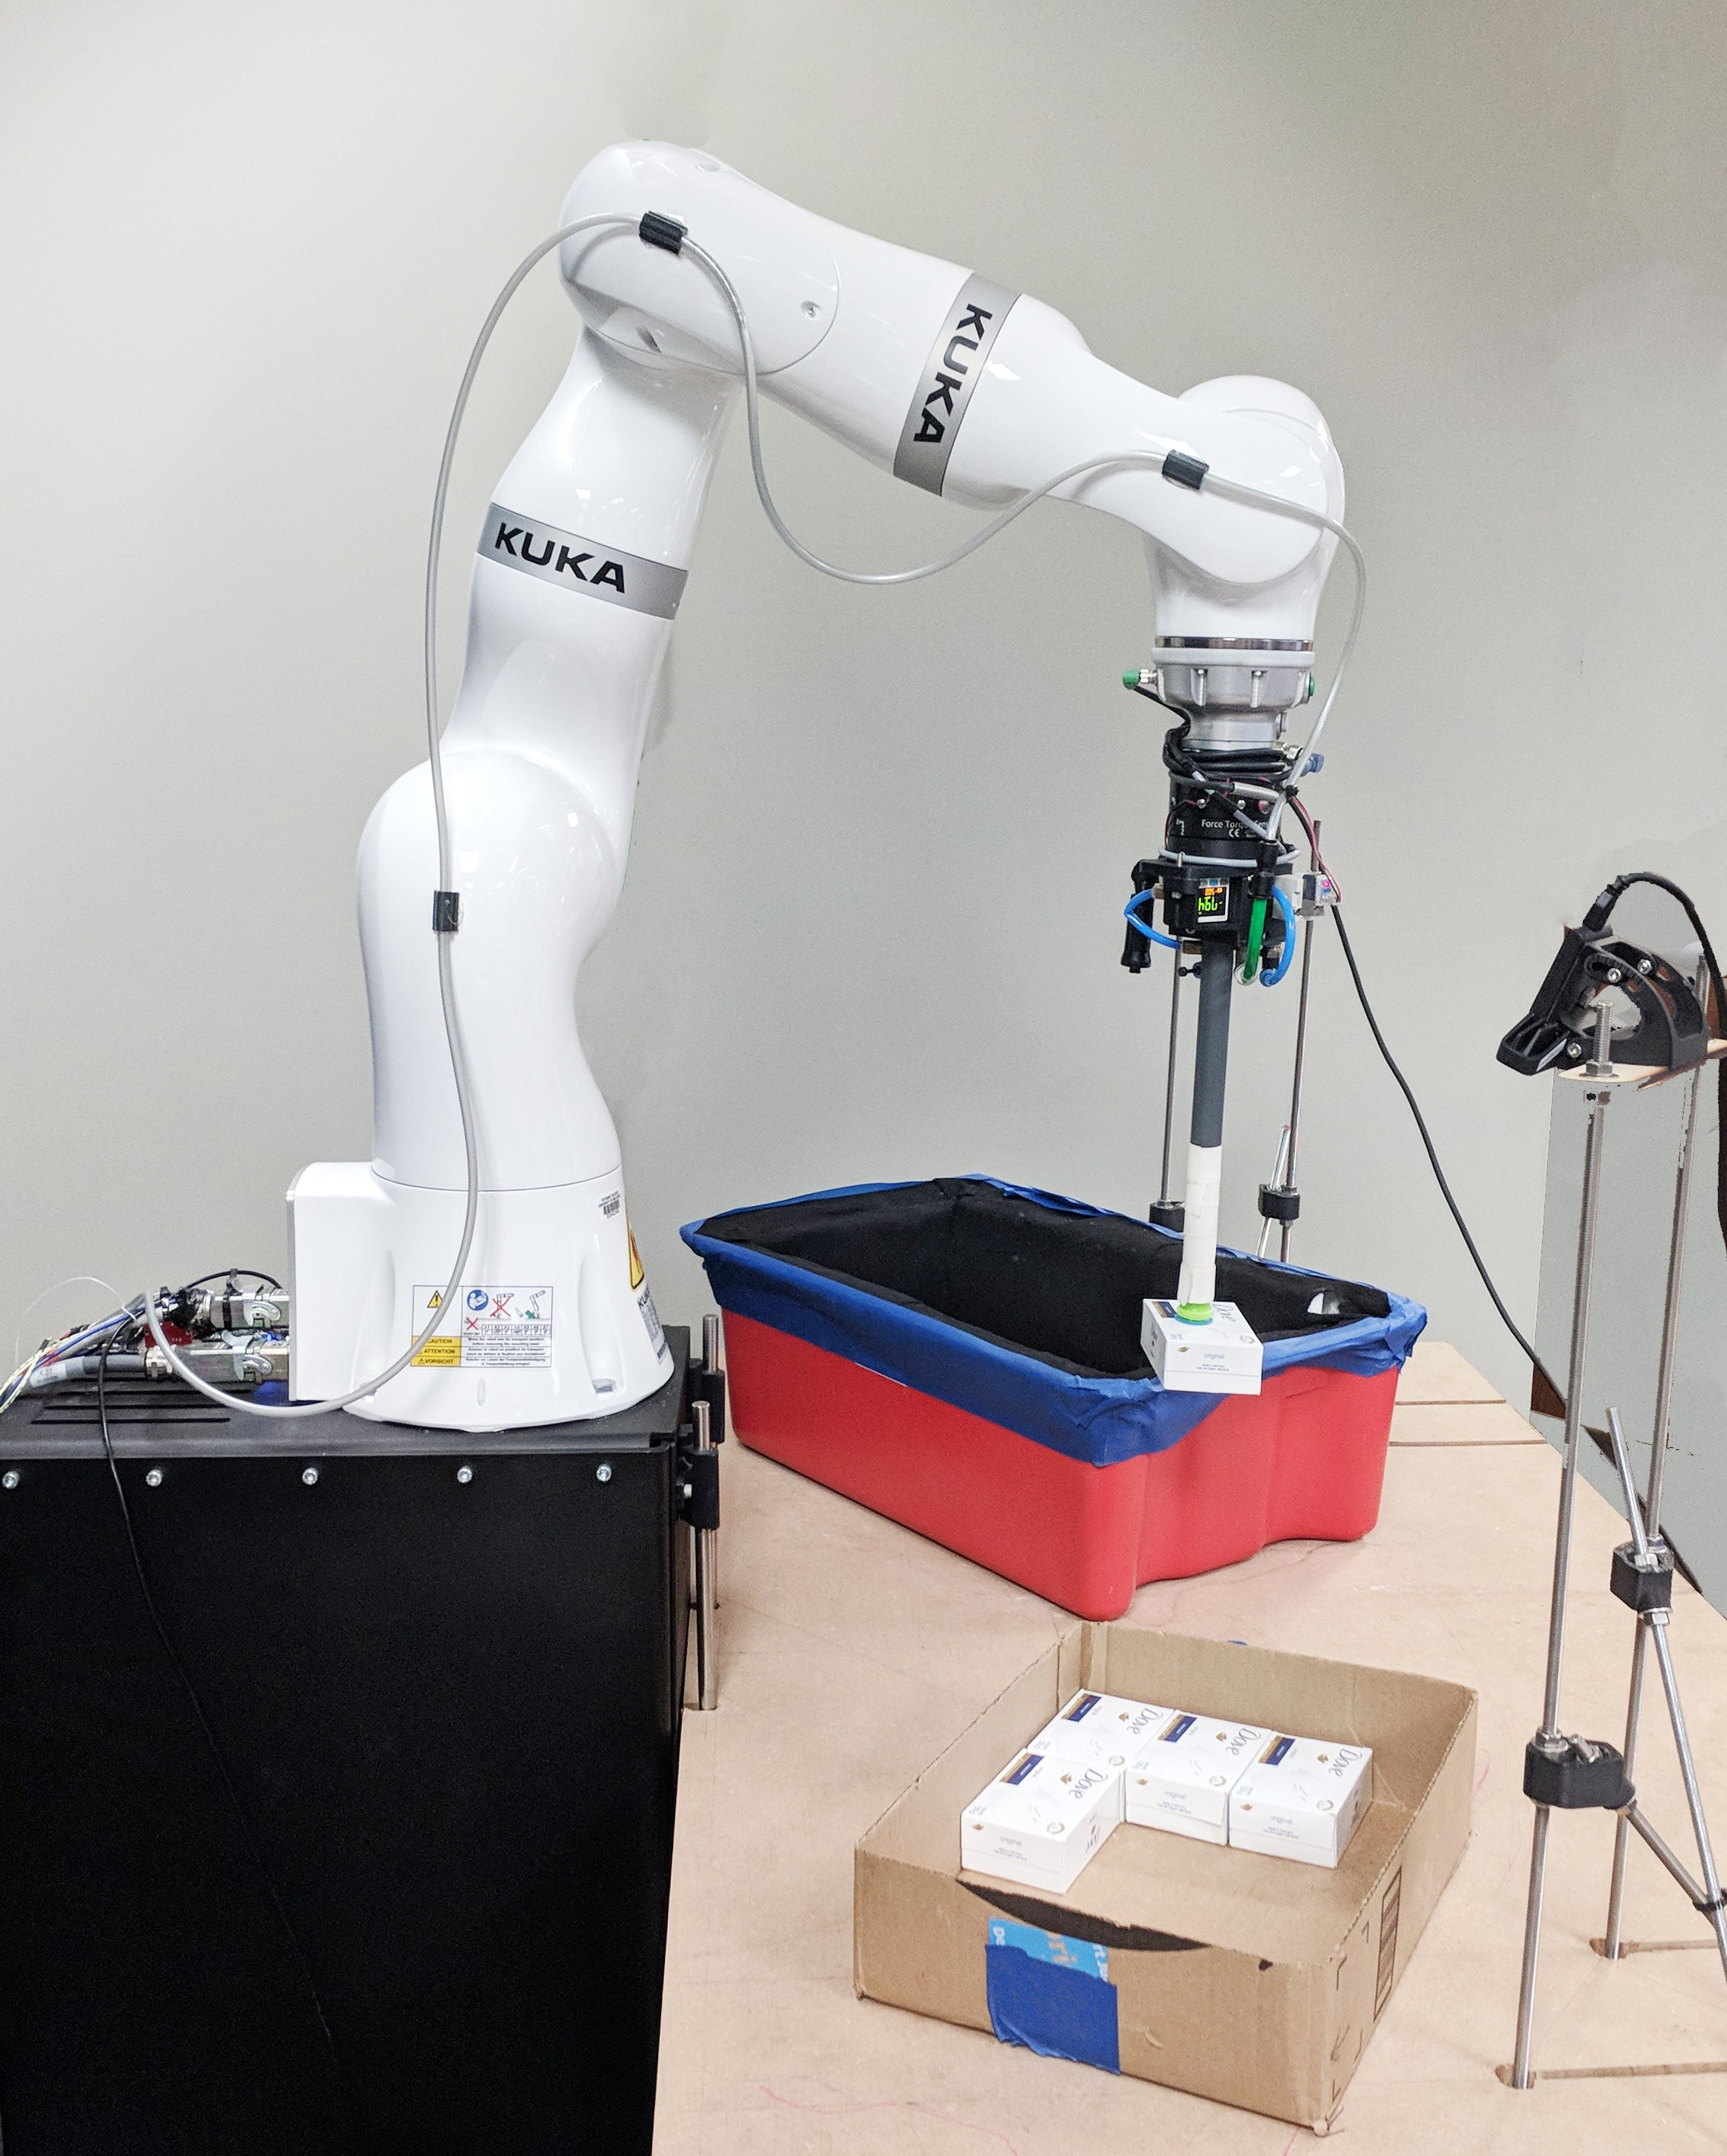
\includegraphics[height=2in]{Figures/robot}
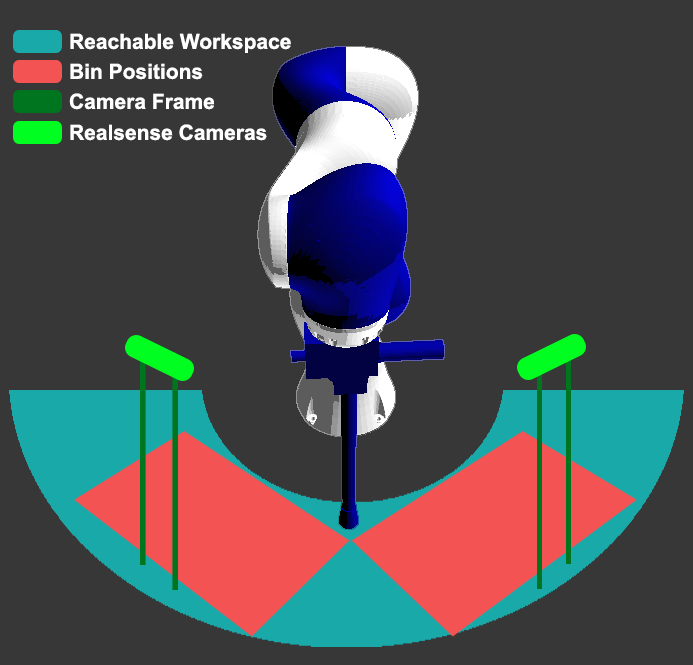
\includegraphics[height=2in]{Figures/workspace}
% \vspace{-0.25in}
\caption{(\textit{Left:}) The product packing problem for cuboid products: initial configuration (top), and achieved goal configuration (bottom). (\textit{Middle:}) Experiments are performed using a {\it Kuka LBR iiwa} arm equipped with a suction-based end-effector and depth-sensing cameras {\it SR300}. (\textit{Right:}) Two bins are within the reachability region of the arm given overhand picks.}
\label{fig:new_setup}
\vspace*{-0.1in}
\end{figure*}

To help narrow the application gap and enable the reliable, fully autonomous execution of such tasks, this paper:

A. Proposes a complete hardware stack and an accompanying software pipeline for developing and testing algorithmic solutions for robot-enabled packing tasks. The hardware setup involves a single robotic arm as shown in Fig. \ref{fig:new_setup}(middle), which depends only on depth-imaging technology to sense its environment. The result is a fully autonomous integrated system for picking objects from unstructured piles and placing them to satisfy a desirable packing arrangement, such as the one shown in Fig.~\ref{fig:new_setup} (left).

B. Explores the use of a suction-based end-effector, which is also treated as a pushing finger, for product packing. The placement of objects, given the packing objective, requires the vacuum-based end-effector to pick objects from specific orientations, which may not be immediately accessible. Nevertheless, the paper demonstrates that the end-effector can still address such challenges in a reliable manner.  

C. Develops and evaluates corrective prehensile and non-prehensile manipulation primitives that increase the pipeline's robustness despite uncertainty regarding the pose of the objects. The uncertainty arises from the end-effector's minimalistic nature and the use of only visual input.  A critical aspect of the primitives is the intentional use of collisions, which exploit the inherent \textit{compliance} of objects, the bins, and the end-effector for enhancing accuracy. Furthermore, the proposed primitives are tightly integrated with sensing to achieve in real-time: 

\begin{myitem}
\item[i)] toppling of objects in the initial unstructured bin to expose a desirable surface of the object for picking; 
\item[ii)] pulling an object towards its target placement while pushing neighboring objects to further pack by operating directly over point cloud data; and 
\item[iii)] real-time monitoring of potential failures and corrective pushing to achieve tight packing.
\end{myitem}

The  evaluation uses the platform of Fig. \ref{fig:new_setup} (middle). The experiments execute the pipeline in real-world scenes and show that the proposed manipulation primitives provide robustness despite the minimalism of the setup.



%Explain some details
% \begin{figure}[t]
% \centering
% 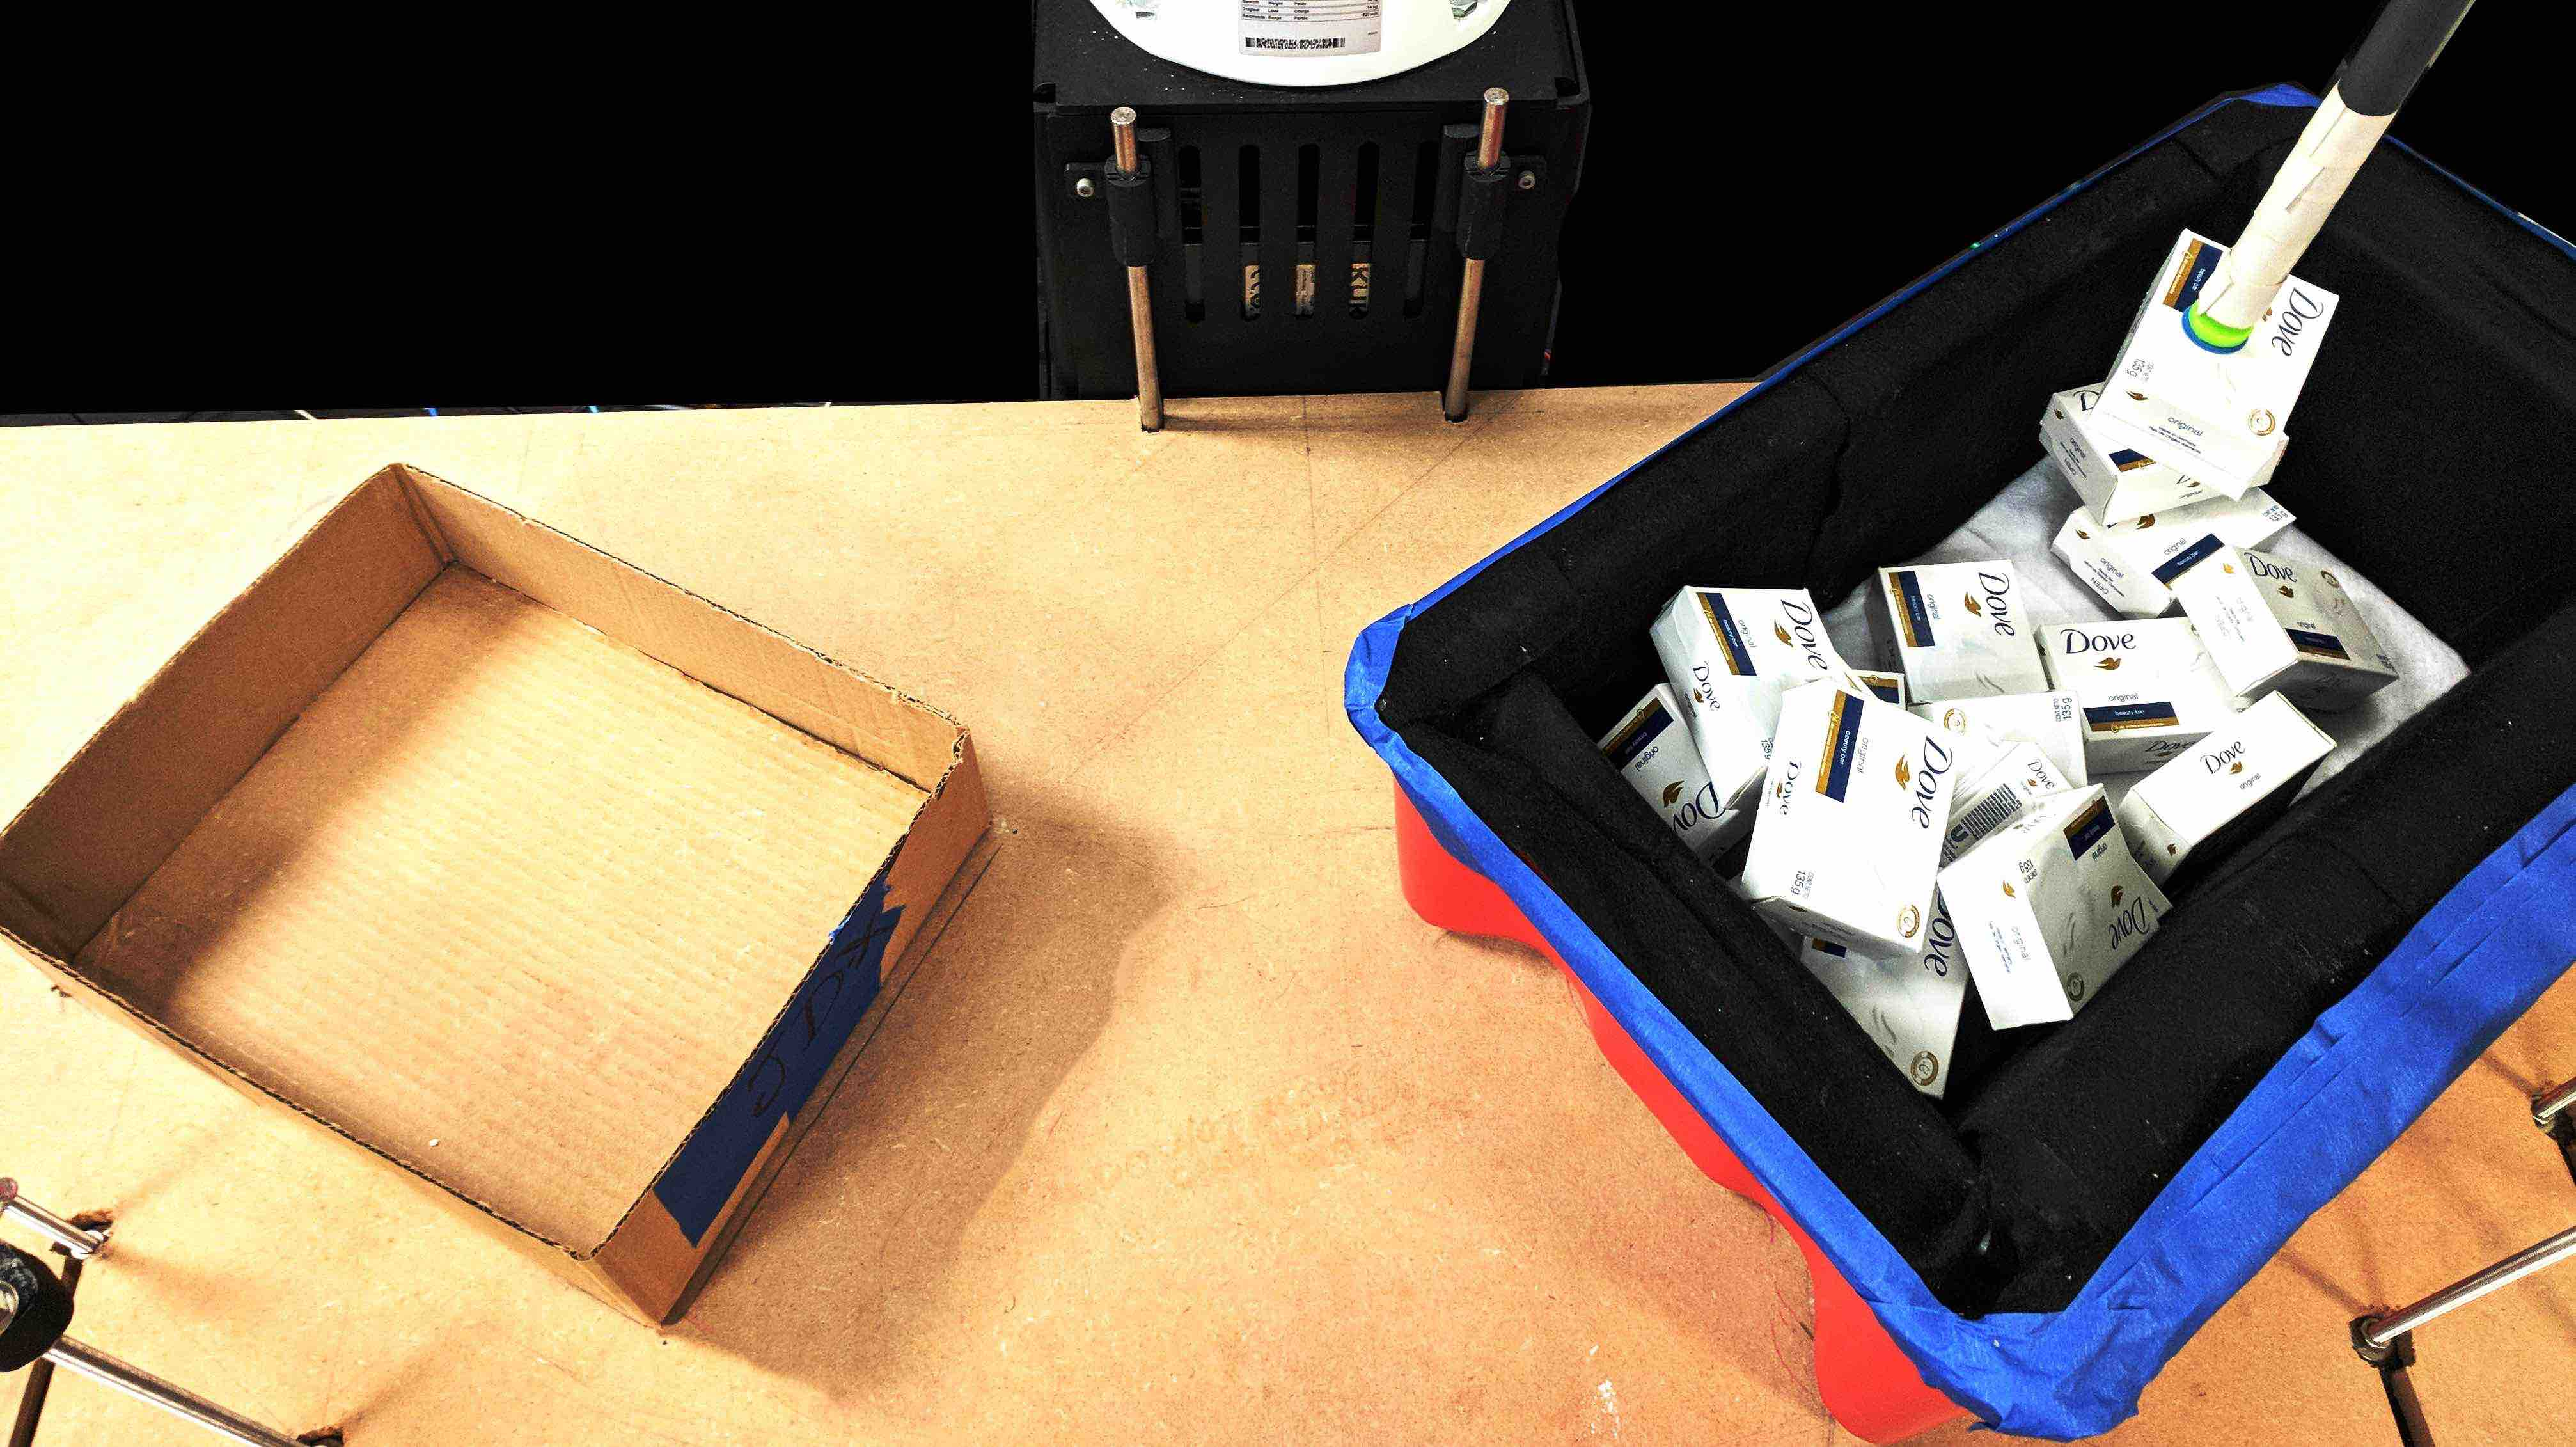
\includegraphics[width=0.225\textwidth]{Figures/initial}
% 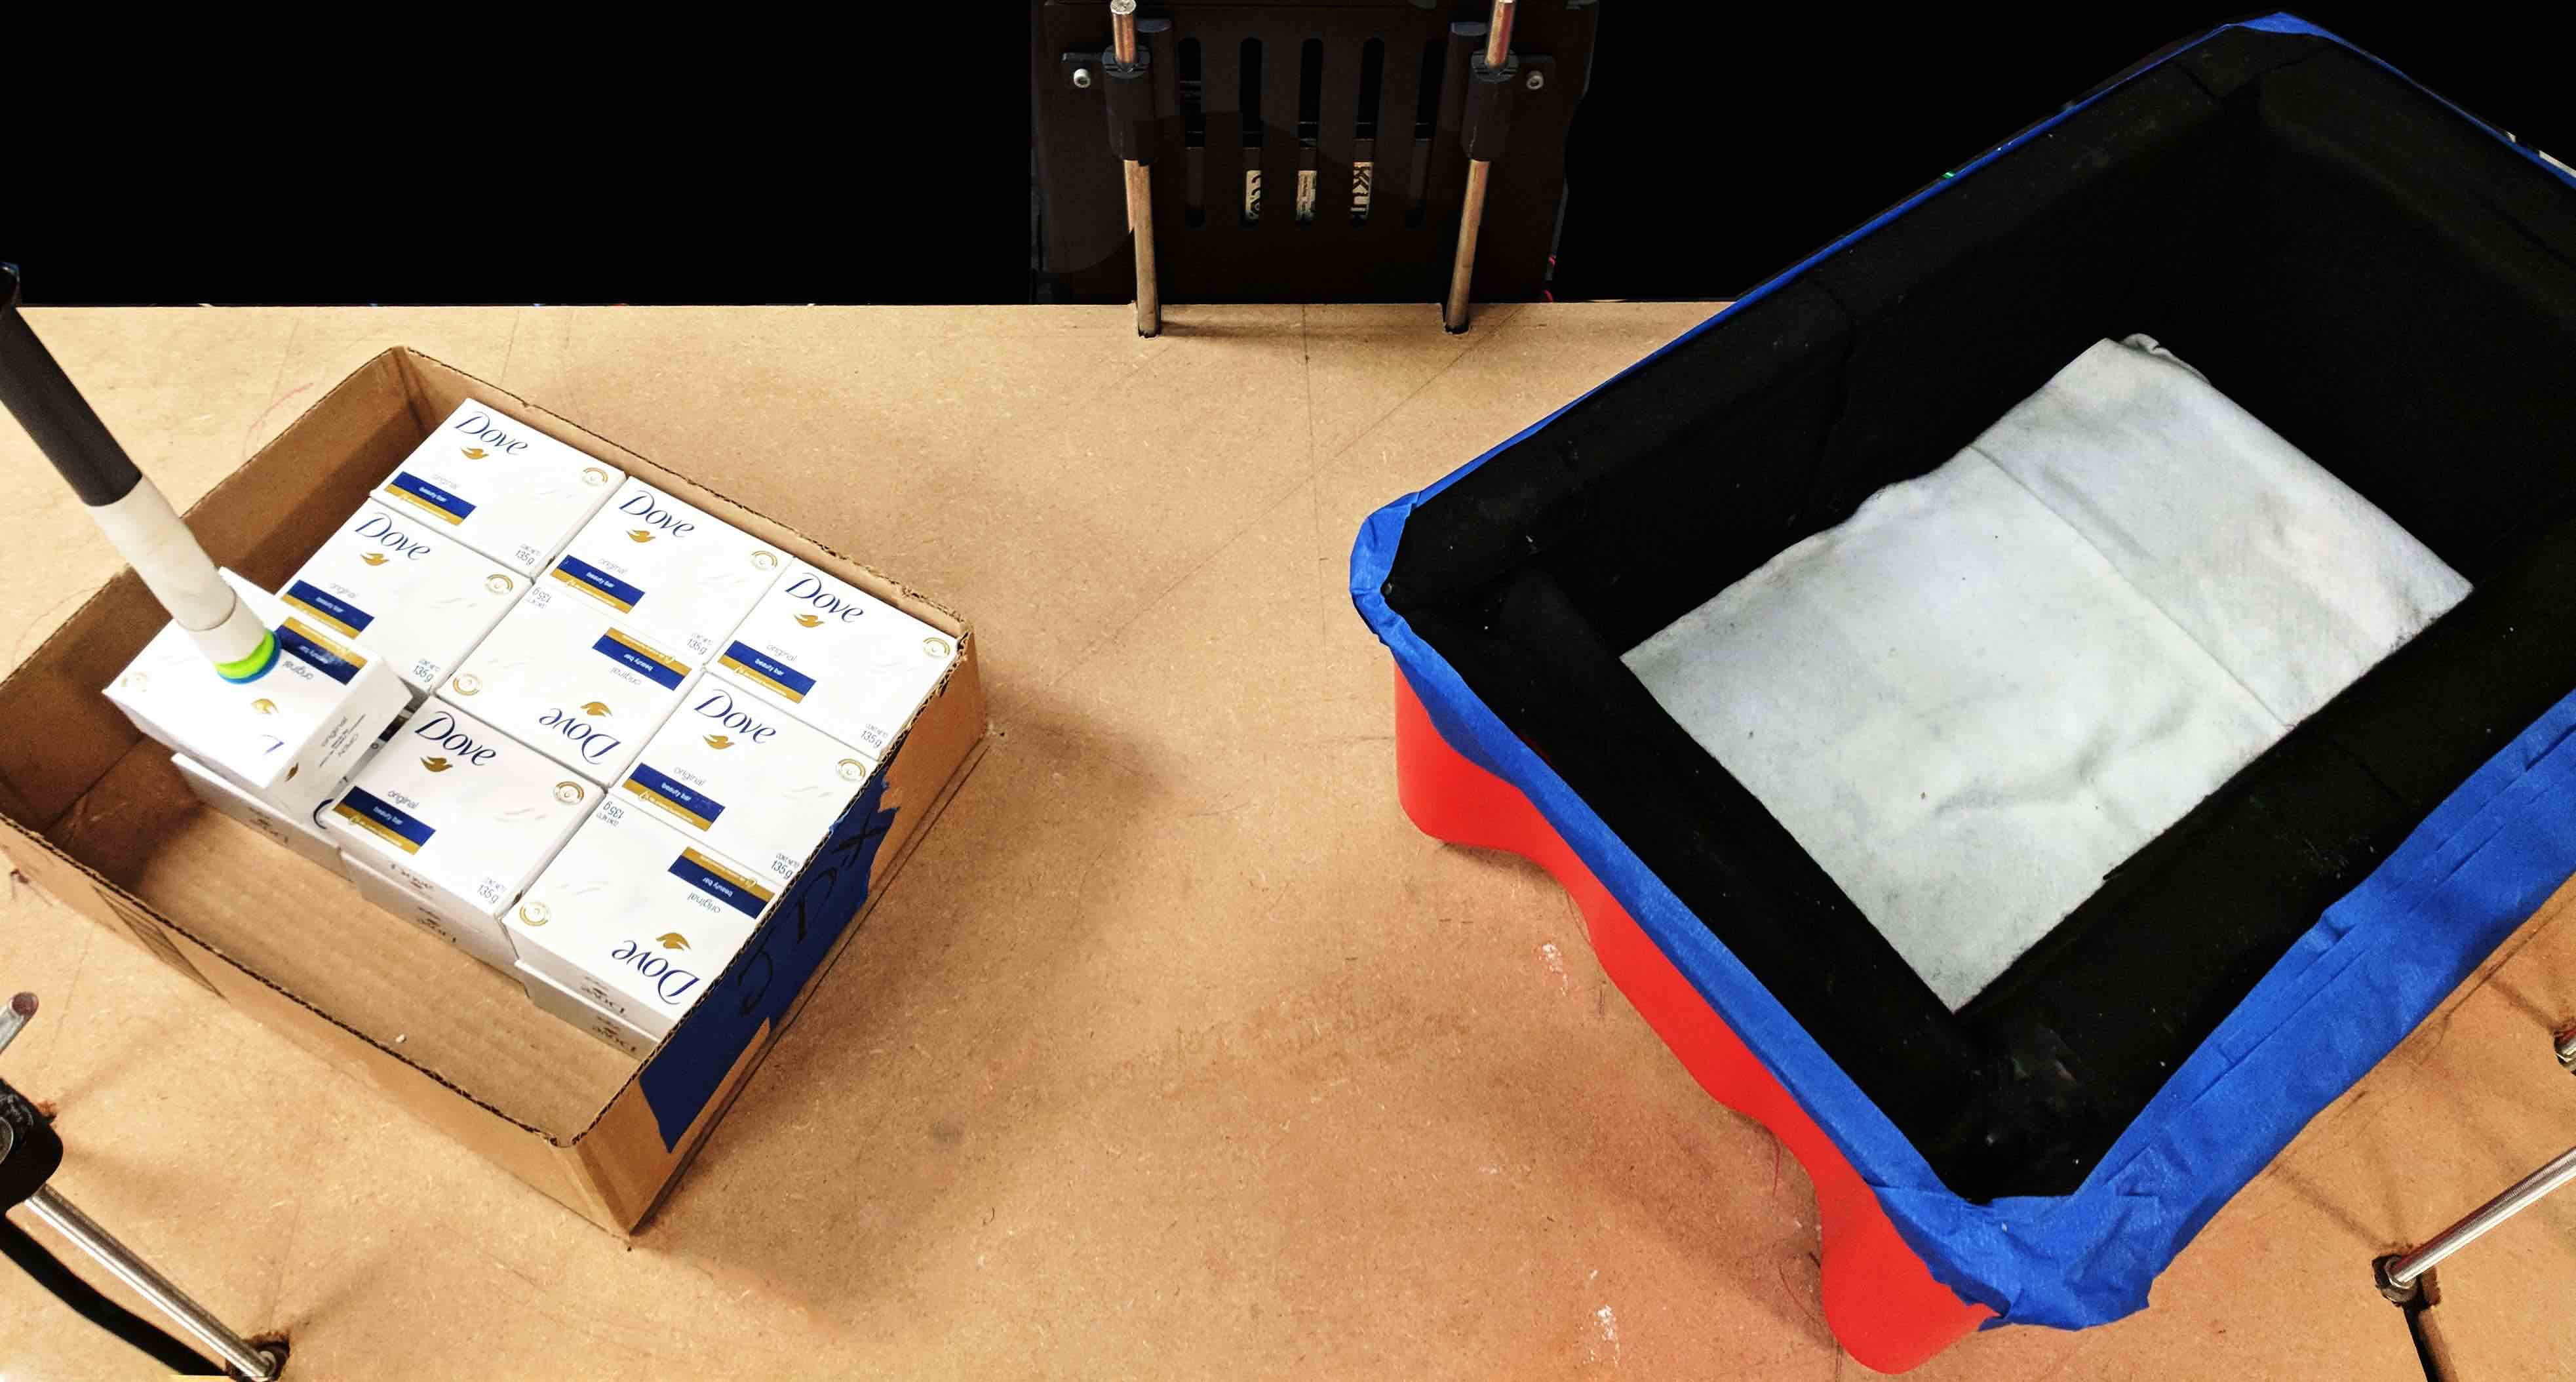
\includegraphics[width=0.235\textwidth]{Figures/final}
% \vspace{-0.1in}
% \caption{The product packing problem for cuboid products: initial configuration (left), and achieved goal configuration (right).}
% %\label{fig:workspace}
% \label{fig:problem_bins}
% \vspace*{-7mm}
% \end{figure}




\rahul{

This paper is an extension of a conference paper \cite{shome2019towards} by the same authors. The current work adds novel content to different aspects of the original study.
% \begin{itemize}
%     \item The coverage of related literature has been expanded to include recent interest and developments that have followed the original work~\cite{shome2019towards}, and specific implementations and use-cases in industrial deployments.
%     \item It expands upon the technical details of the primitives presented in the conference paper in Section~\ref{section:Pipeline}.  
%     \begin{itemize}
%         \item The geometric reasoning in the computation of the toppling primitive has been highlighted, along with diagrammatic steps.
%         \item A novel extension to the adaptive pushing primitive has been added to allow its application to problem instances with no additional clearance, as long as there is sufficient compliance.
%         \item Pseudocode and expository descriptions have been added to all the primitives.
%     \end{itemize}
%     \item The evaluation Section~\ref{section:evaluation} has been significantly expanded, with a focus on simulations.
%     \begin{itemize}
%         \item A simulator is developed that automatically generates RGB-D data corresponding to placement scenarios and mimics the behavior of compliant pushing actions over the specified control inputs. The simulator will be made publicly available to the community to facilitate research along this direction. 
%         \item Ablation experiments have been added to test a) the robustness of the proposed manipulation primitives against different levels of simulated noise (Fig. 10, 15), and b) the impact of underlying parameters and simplifying assumptions on their efficiency (Fig. 11, 12, 16) in simulation
%     \end{itemize}
%     \item Finally, additional demonstrations, which were performed on the real robot to further showcase extended capabilities of the originally proposed system. The demonstrations correspond to 
%     \begin{itemize}
%         \item an extension of adaptive pushing that solves hard scenarios where the size of the box is exactly the size of placement volume
%         \item handling a pile with different objects in the picking bin and packing them into separate boxes, one after the other
%         \item toppling the object to the narrow side where the final configuration is less stable than the initial one
%     \end{itemize}
%         % Section V expands upon the technical details of the proposed solution with additional supporting figures (Fig. 5, 6, 8) and algorithmic blocks (Alg. 1, 2). In addition to the simulation results, Section VI also evaluates the packing efficiency of real-world experiments in terms of the final object poses. This metric depends less on the quality of the sensor data. 
% \end{itemize}

Building on the extensive real-world experiments that validated the proposed pipeline, a robust simulation framework has been added in the current work to allow more controlled evaluation and testing of the individual primitives. A key aspect of the simulator is that it allows the modeling of high-fidelity RGBD sensor information (through \textit{Blender}), along with modeling of the compliance of the interactions between the end-effector suction cup, and the different objects that arise from pushing, and fine-correcting them. A simulator can automatically generates RGB-D data corresponding to placement scenarios and mimics the behavior of compliant pushing actions over the specified control inputs. The simulator has been made publicly available\footnote{\url{https://robotpacking.org/simulator.html}} to the community to facilitate research along this direction. The extensible and modular nature of the interface to the simulator is expected to aid researchers and industry partners interested in robust robotic packing. Ablation experiments have been added to test a) the robustness of the proposed manipulation primitives against different levels of simulated noise, and b) the impact of underlying parameters and simplifying assumptions on their efficiency in simulation.

A novel extension to the adaptive pushing primitive has been added to allow its application to problem instances with no additional clearance, as long as there is sufficient compliance. A real world demonstrations to show the efficacy of this primitive has additionally been included in Section~\ref{section:evaluation}. This is meant to address problems instances where the size of the box is exactly the size of placement volume. The key spirit of the proposed methods of leveraging the compliance of the environment allows the extended variant of adaptive pushing to work even in these hard scenarios.

Additional demonstrations, which were performed on the real robot to further showcase extended capabilities of the originally proposed system. The demonstrations correspond to a) toppling the object to the narrow side where the final configuration is less stable than the initial one, and b) handling a pile with different objects in the picking bin and packing them into separate boxes, one after the other. 

In terms of additional content inside the text, the coverage of related literature has been expanded to include recent interest and developments that have followed the original work~\cite{shome2019towards}, and specific implementations and use-cases in industrial deployments. It expands upon the technical details of the primitives presented in the conference paper in Section~\ref{section:Pipeline}. The geometric reasoning in the computation of the toppling primitive has been highlighted, along with diagrammatic steps. Pseudocode and expository descriptions have been added to all the primitives.


}

% \begin{comment}
% There has been significant interest in the deployment of robotic systems in warehouse automation~\cite{correll2016analysis, baker2007exploration, d2012guest}. Typically robots have been used for large scale industrial setups to perform repetitive tasks in highly structured environments, as in automobile manufacturing. Recently, there is a push to expand the applications of robotic arms in less structured settings that arise in order fulfillment as well as warehouse packing tasks. The problem of packing boxes into bins arises in a vast spectrum of typical warehouse applications. This motivates a closer inspection of the problem of tightly packing cuboidal objects, that are a compelling use-case of modern e-commerce and order fulfillment. \\
% Prior work~\cite{correll2016analysis,166} has investigated the importance of careful design choices in terms of end-effector modalities, perception systems and planning methods that are appropriate for the problem. The current work focuses on a specific challenge involving two bins in the robot's reachable workspace on a tabletop, where the objective is to pick up every object from the source bin, and transfer all of them to the target bin, as fast and robustly as possible.\\
% \textbf{JJ: The above Might be somewhat redundant; needs editing/removing. Some might go to the related work section.}
% \end{comment}

% \begin{figure}[t]
% \centering
% 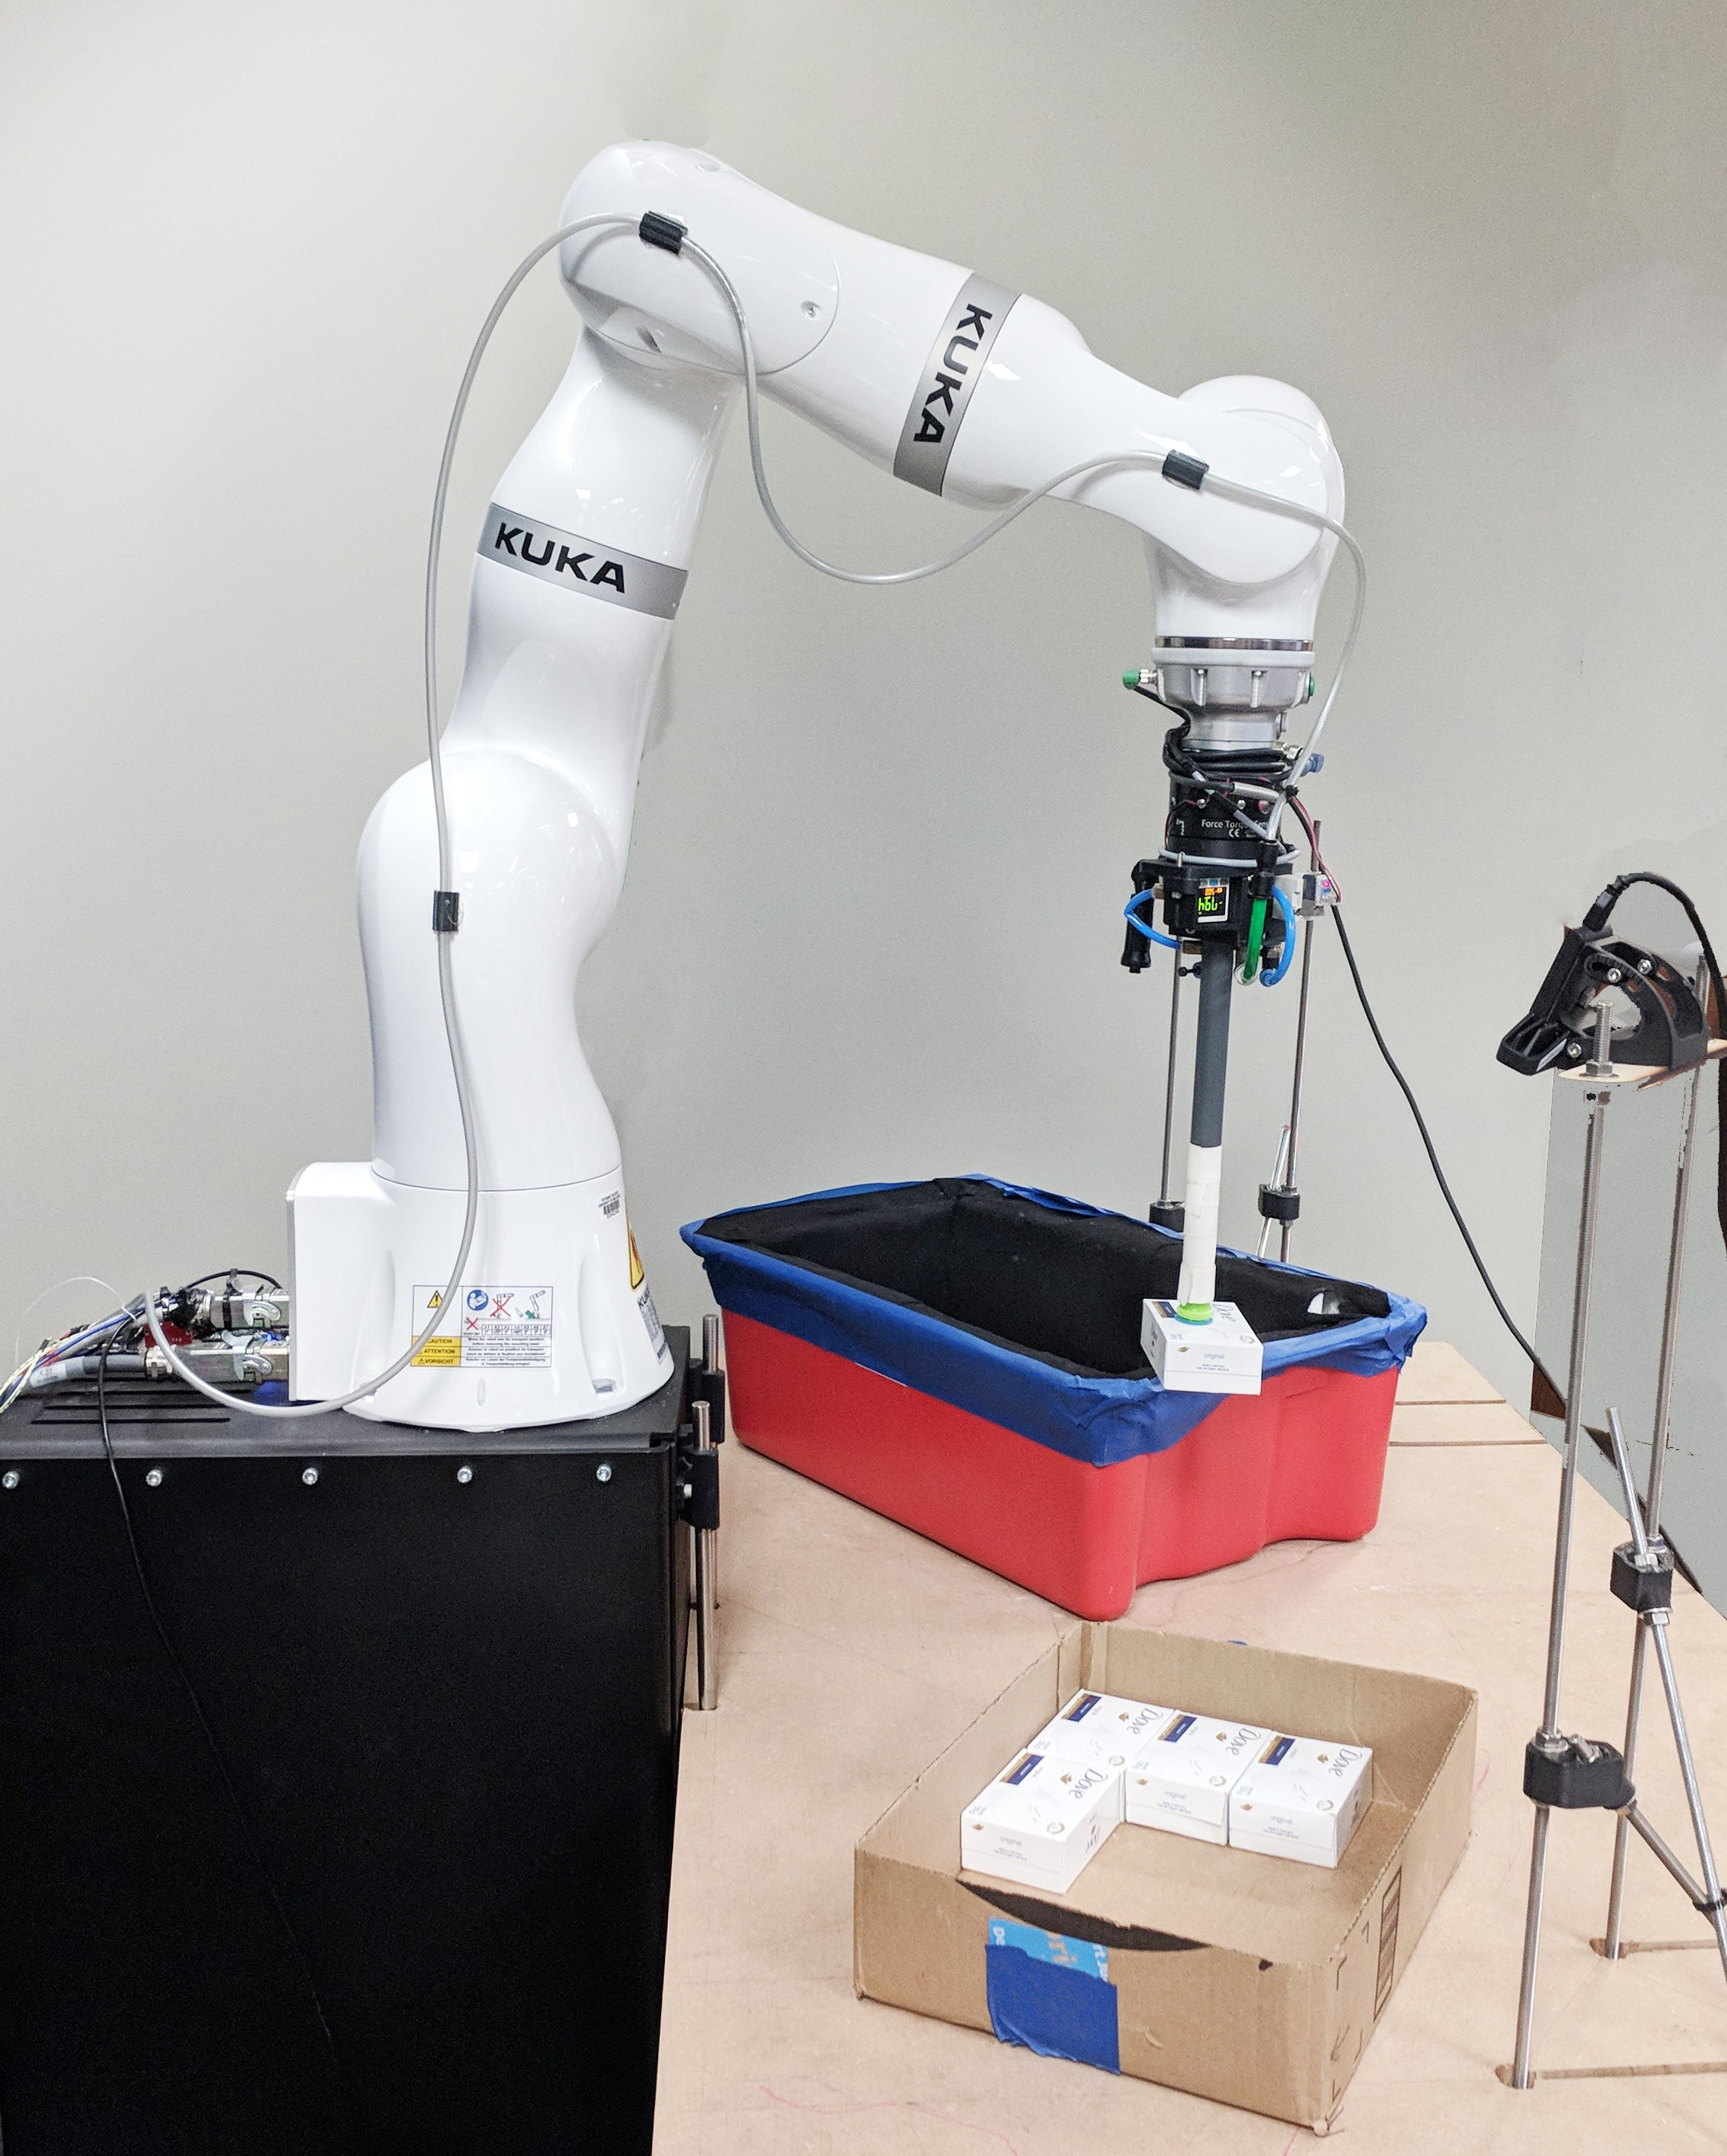
\includegraphics[width=0.208\textwidth]{Figures/robot}
% 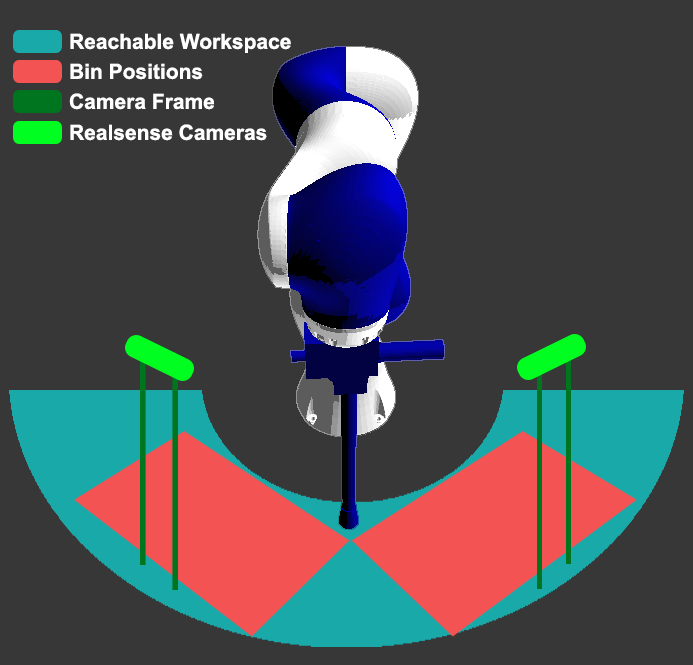
\includegraphics[width=0.27\textwidth]{Figures/workspace}
% \vspace{-0.25in}
% \caption{Experiments are performed using a {\it Kuka LBR iiwa} arm equipped with a suction-based end-effector and depth-sensing cameras {\it SR300}. Two bins are within the reachability region of the arm given overhand picks.}
% %\label{fig:workspace}
% \label{fig:setup}
% \vspace*{-0.1in}
% \end{figure}

% - Using environment and collision to do toppling in multiple ways
% - Adaptive path planning based directly on point cloud for aligning objects 
% - Using corrective motion to achieve tight packing 
% - Robustness via execution monitoring 

%======================================================================================


%A solution to such a problem is closely intertwined with the accuracy and success of a large set of components like sensing, grasp generation, motion planning, and task planning. The current work focuses on the task planning strategies that can push the success of the overall task, without making any assumptions of the perception, grasping generation or motion planning steps. The paper describes the task planning solution employed that stacks a hierarchy of strategies of increasing complexity, and robustness, to attempt to efficiently solve the problem. The chief concern in the bin-packing task is the practical source of perception and execution errors. When dealing with perfectly packing cuboids, the margin of error is very low. Naive strategies are cheaper to compute and execute but are typically more error prone. This motivates the use of higher level reasoning, including push primitives that ensure robust packing, regrasping strategies to guarantee grasps for every object, and scene corrections in the target bin to prevent future failures. 
